\documentclass{beamer}
\usetheme{Warsaw}
%\usetheme{default}
\usepackage[utf8]{inputenc}
\usepackage[utf8x]{inputenc}
%\usepackage{paralist}
\title{Um algoritmo evolucion\'{a}rio h\'{i}brido baseado na fertiliza\c{c}\~{a}o in vitro para solucionar problemas de escalonamento job-shop}
\author{\'{E}werton Carlos de Ara\'{u}jo Assis}
\date{Dezembro 2011}
\begin{document}

\begin{frame}[plain] 
  \titlepage
\end{frame}

\begin{frame}
  \tableofcontents[sections={1-3}]
\end{frame}

\begin{frame}
  \tableofcontents[sections={4-6}]
\end{frame}

\begin{frame}
  \tableofcontents[sections={7-9}]
\end{frame}

\section{Introdução}
\begin{frame}{Heur\'{i}sticas e metaheur\'{i}sticas como meios de resolucionar problemas de escalonamento job-shop}
\begin{itemize}
\item<1-> Complexidade dos problemas de escalonamento job-shop e demais problemas de otimiza\c{c}\~{a}o
\item<2-> Import\^{a}ncia das heur\'{i}sticas e metaheur\'{i}sticas em problemas de otimiza\c{c}\~{a}o
\item<3-> Necessidade de hibridiza\c{c}\~{a}o das metaheur\'{i}sticas
\item<4-> Estudos de caso: efetividade e efici\^{e}ncia de uma solu\c{c}\~{a}o metaheur\'{i}stica
\end{itemize}
\end{frame}

\subsection{Objetivos}
\begin{frame}{Objetivos do presente trabalho}
\begin{itemize}
\item<1-> Identificar problemas de escalonamento job-shop (PEJS) e suas defini\c{c}\~{o}es
\item<2-> Identificar heur\'{i}sticas e metaheur\'{i}sticas utilizadas em PEJS
\item<3-> Definir uma solu\c{c}\~{a}o metaheur\'{i}stica h\'{i}brida baseada na fertiliza\c{c}\~{a}o in vitro (FIV-AG)
\item<4-> Analisar a solu\c{c}\~{a}o algor\'{i}tmica constru\'{i}da e sua efetividade
\end{itemize}
\end{frame}

\section{Problemas de escalonamento job-shop}
\begin{frame}{Problemas de escalonamento job-shop (PEJS)}
Definição formal de um problema de escalonamento job-shop:
\begin{itemize}
\item<1-> São dadas $n$ tarefas (ou \textit{jobs}) $ \{ J_{1}, J_{2}, ..., J_{n} \} $ a serem processadas por $m$ m\'{a}quinas 
$\{ M_{1}, M_{2}, ..., M_{m} \}$ --- cada tarefa deve ser processada por cada m\'{a}quina uma \'{u}nica vez
\item<2-> O processamanto de uma tarefa em uma m\'{a}quina \'{e} denominado opera\c{c}\~{a}o: a opera\c{c}\~{a}o da tarefa $i$
na m\'{a}quina $j$ \'{e} denotada por $o_{ij}$
\item<3-> Cada tarefa $i$  ($J_{i}$) apresenta um tempo de processamento para cada m\'{a}quina, i.e. para cada opera\c{c}\~{a}o
$o_{ij}$ h\'{a} um tempo de processamento $p_{ij}$
\end{itemize}
\end{frame}
\begin{frame}{Problemas de escalonamento job-shop (PEJS)}
\begin{itemize}
\item<1-> Restri\c{c}\~{o}es tecnol\'{o}gicas determinam a ordem de processamento de cada tarefa atrav\'{e}s das $m$ m\'{a}quinas
\item<2-> As tarefas em um problema de escalonamento job-shop n\~{a}o compartilham uma mesma ordem de processamento atrav\'{e}s
das m\'{a}quinas
\end{itemize}
\end{frame}
\begin{frame}{Problemas de escalonamento job-shop (PEJS)}
Considerações relativas à definição:
\begin{itemize}
\item<1-> Necessidade de construir um escalonador de tarefas de forma a agendar as $n$ tarefas atrav\'{e}s das $m$ m\'{a}quinas
a partir de critérios de otimização estabelecidos
\item<2-> O problema de escalonamento job-shop \'{e} considerado um problema numericamente intrat\'{a}vel, NP-dif\'{i}cil
(para $m \geq 2$) \cite{French1982} e que apresenta um limite superior de $(n!)^{m}$ solu\c{c}\~{o}es poss\'{i}veis
\end{itemize}
\end{frame}
\begin{frame}{Problemas de escalonamento job-shop (PEJS)}
\begin{center}
  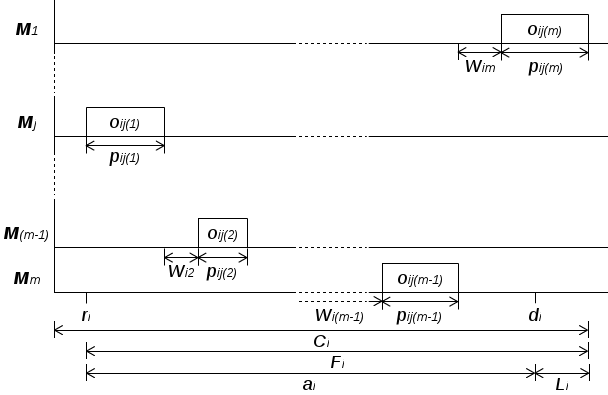
\includegraphics[width=0.7\textwidth]{../imgs/gantt.png}
\end{center}
\end{frame}

\subsection{Critérios de otimização}
\begin{frame}{Critérios de otimização}
\begin{itemize}
\item<1-> O crit\'{e}rio b\'{a}sico tem como objetivo minimizar o $C_{max}$ (\textit{makespan}), i.e. minimizar o tempo total da
tarefa de maior tempo de processamento
\end{itemize}
\begin{center}
\paragraph{\indent $C_{i}$ \'{e} o tempo total de processamento da tarefa $J_{i}$, ou $C_{i} = r_{i}
+ \sum_{k=1}^{m}(W_{ik} + p_{ij(k)})$}
\end{center}
\begin{description}
\item[$r_{i}$] determina a partir de quanto tempo ou em qual momento a tarefa $i$ ($J_{i}$) estar\'{a} dispon\'{i}vel para
processamento pelas $m$ m\'{a}quinas da oficina
\item[$W_{ik}$] \'{e} o tempo de espera da tarefa $J_{i}$ no processamento da opera\c{c}\~{a}o $k$
\end{description}
\end{frame}
\begin{frame}{Critérios de otimização}
\begin{itemize}
\item<1-> A minimiza\c{c}\~{a}o do valor $F_{max}$ tem por objetivo minimizar o tempo tempo gasto pelas tarefas na oficina
\end{itemize}
\begin{center}
\paragraph{$F_{max}$ o tempo total de processamento da tarefa que permaneceu por mais tempo na oficina}
\end{center}
\begin{description}
\item[$F_{i}$] é o tempo de processamento da tarefa $i$ a partir do instante que esta encontra-se na oficina ($F_{i} = C_{i} - r_{i}$)
\end{description}
\end{frame}
\begin{frame}{Crit\'{e}rios baseados na data de entrega}
\begin{itemize}
\item<1-> Minimiza\c{c}\~{a}o do valor $T_{max}$ \'{e} apropriada em contextos nos quais o atraso no processamento de tarefas
apresenta alguma penalidade
\item<2-> Minimiza\c{c}\~{a}o do valor $E_{max}$ \'{e} apropriada nos contextos em que h\'{a} um benef\'{i}cio ao antecipar-se
o processamento das tarefas
\end{itemize}
\begin{description}
\item[$d_{i}$] \'{e} a data de vencimento ou a data de entrega da tarefa $i$, o tempo ideal para que a tarefa seja completada;
\item[$T_{i}$] $T_{i} = \textit{max}\{C_{i} - d_{i} , 0\}$, o atraso da tarefa $J_{i}$; e
\item[$E_{i}$] $E_{i} = \textit{max}\{d_{i} - C_{i} , 0\}$, a atencipa\c{c}\~{a}o da tarefa $J_{i}$.
\end{description}
\end{frame}
\begin{frame}{Crit\'{e}rios baseados na data de entrega}
\begin{itemize}
\item<1-> Seja $n_{T}$ o número de tarefas atrasadas, a minimização do valor $n_{T}$ tem o propósito de diminuir o número de
tarefas atrasadas
\end{itemize}
\end{frame}
\begin{frame}{Crit\'{e}rios baseados em custos}
\begin{description}
\item[$N_{w(t)}$] o n\'{u}mero de tarefas esperando para serem processadas por alguma m\'{a}quina ou tarefas que ainda n\~{a}o est\~{a}o prontas
para serem processadas
\item[$N_{p(t)}$] o n\'{u}mero de tarefas sendo processadas no tempo $t$
\item[$N_{c(t)}$] o n\'{u}mero de tarefas completadas no tempo $t$
\item[$N_{u(t)}$] o n\'{u}mero de tarefas a serem ainda completadas no tempo $t$
\end{description}
\end{frame}
\begin{frame}{Crit\'{e}rios baseados em custos}
\begin{itemize}
\item<1-> Minimizar o n\'{u}mero m\'{e}dio de tarefas esperando para serem processadas ($\bar{N}_{w}$) ou minimizar o n\'{u}mero m\'{e}dio de
tarefas n\~{a}o completadas ($\bar{N}_{u}$) de forma a minimizar os custos de invent\'{a}rio
\item<2-> Minimizar o n\'{u}mero m\'{e}dio de tarefas completadas ($\bar{N}_{c}$), de forma a reduzir os custos dos bens produzidos
\item<3-> Maximizar o n\'{u}mero m\'{e}dio de tarefas sendo processadas ($\bar{N}_{p}$) com o intuito de realizar um uso eficiente das m\'{a}quinas
\end{itemize}
\end{frame}

\subsection{Pressupostos em problemas de escalonamento job-shop}
\begin{frame}{Pressupostos em problemas de escalonamento job-shop}
\begin{itemize}
\item<1-> Cada tarefa \'{e} uma entidade
\item<2-> N\~{a}o existe preemp\c{c}\~{a}o
\item<3-> Cada tarefa \'{e} constitu\'{i}da de $m$ opera\c{c}\~{o}es distintas, uma para cada m\'{a}quina
\item<4-> Tarefas n\~{a}o s\~{a}o canceladas
\end{itemize}
\end{frame}
\begin{frame}{Pressupostos em problemas de escalonamento job-shop}
\begin{itemize}
\item<1-> O tempo de processamento \'{e} independente da agenda constru\'{i}da
\item<2-> Tarefas podem ter que esperar para serem processadas
\item<3-> Existe apenas um \'{u}nico tipo de cada m\'{a}quina
\item<4-> M\'{a}quinas podem estar ociosas
\end{itemize}
\end{frame}
\begin{frame}{Pressupostos em problemas de escalonamento job-shop}
\begin{itemize}
\item<1-> As m\'{a}quinas n\~{a}o podem processar qualquer tarefa mais de uma vez
\item<2-> As m\'{a}quinas da oficina est\~{a}o sempre dispon\'{i}veis para processamento das tarefas
\item<3-> As restri\c{c}\~{o}es tecnol\'{o}gicas s\~{a}o imut\'{a}veis e previamente conhecidas
\item<4-> N\~{a}o existe aleatoriedade
\end{itemize}
\end{frame}

\subsection{Extens\~{o}es \`{a} defini\c{c}\~{a}o tradicional}
\begin{frame}{Extens\~{o}es \`{a} defini\c{c}\~{a}o tradicional}
\begin{description}
\item[PEJS flex\'{i}vel] al\'{e}m de determinar a ordem de execu\c{c}\~{a}o das tarefas, o escalonador deve
determinar em qual das m\'{a}quinas determinada tarefa ser\'{a} executada em dado momento
\item[PEJS multi-objetivo] estabelecem mais de um crit\'{e}rio de otimiza\c{c}\~{a}o no modelo do problema a ser solucionado
\end{description}
\end{frame}

\section{Solu\c{c}\~{o}es heur\'{i}sticas e metaheur\'{i}sticas}
\begin{frame}{Solu\c{c}\~{o}es heur\'{i}sticas e metaheur\'{i}sticas}
\begin{description}
\item[Heurística] ``a arte de descobrir novas estrat\'{e}gias (...) para solucionar problemas'' (tradu\c{c}\~{a}o livre) \cite{Talbi2009};
\item[Metaheur\'{i}sticas] ``m\'{e}todos de solu\c{c}\~{a}o que orquestram uma intera\c{c}\~{a}o entre procedimentos de melhora local
e estrat\'{e}gias de alto n\'{i}vel com o fim de criar um processo capaz de escapar de \'{o}timos locais e realizar uma busca robusta
em um espa\c{c}o de busca'' (tradu\c{c}\~{a}o livre) \cite{Gendreau2010}.
\end{description}
\end{frame}
\begin{frame}{Solu\c{c}\~{o}es heur\'{i}sticas e metaheur\'{i}sticas}
Metaheurísticas geralmente utilizadas como meio de resolucionar problemas de escalonamento job-shop:
\begin{itemize}
\item<1-> algoritmos genéticos;
\item<2-> algoritmos meméticos;
\item<3-> \textit{particle swarm optimization};
\item<4-> \textit{simulated annealing};
\item<5-> \textit{ant colony optmization};
\item<6-> \textit{variable neighborhood search}; e
\item<7-> busca tabu.
\end{itemize}
\end{frame}

\subsection{Padrões identificados nos métodos de solução metaheurísticos}
\begin{frame}{Padrões identificados nos métodos de solução metaheurísticos}
\begin{itemize}
\item<1-> M\'{e}todos metaheur\'{i}sticos híbridos
\item<2-> As 82 inst\^{a}ncias dispon\'{i}veis na OR-Library \cite{OrLibrary} e as 80 inst\^{a}ncias de Taillard \cite{Taillard1993}
s\~{a}o frequentemente utilizadas como meios para estabelecer-se a qualidade da solu\c{c}\~{a}o proposta frente aos resultados obtidos
por outras solu\c{c}\~{o}es
\item<3-> Representação da solução através de \textit{random-keys}, ou chaves aleatórias. Representação centrada na ordem de processamento
das operações
\end{itemize}
\end{frame}
\begin{frame}{Padrões identificados nos métodos de solução metaheurísticos}
\begin{itemize}
\item<1-> Uso de opera\c{c}\~{o}es de permuta\c{c}\~{a}o como operador de busca local ou como operador de muta\c{c}\~{a}o em algoritmos
evolucionários. Operadores de permutação:
\begin{itemize}
\item<2-> inser\c{c}\~{a}o;
\item<3-> invers\~{a}o (geralmente de elementos adjacentes);
\item<4-> permuta\c{c}\~{a}o ou troca de elementos em posi\c{c}\~{o}es distintas; e
\item<5-> movimento de longa dist\^{a}ncia (mover uma sequ\^{e}ncia de elementos a uma determinada posi\c{c}\~{a}o ou dire\c{c}\~{a}o).
\end{itemize}
\end{itemize}
\end{frame}

\section{Solução metaheurística evolucionária}
\begin{frame}{Solução metaheurística evolucionária}
Componentes de uma solução algorítmica evolucionária:
\begin{itemize}
\item<1-> Representa\c{c}\~{a}o da solu\c{c}\~{a}o do problema como um indiv\'{i}duo (solu\c{c}\~{a}o--indiv\'{i}duo)
\item<2-> População de indivíduos--soluções e desenvolvimento geracional dessa população
\item<3-> Conceitos biol\'{o}gicos como evolu\c{c}\~{a}o, aptid\~{a}o, recombina\c{c}\~{a}o e muta\c{c}\~{a}o gen\'{e}tica influenciam
essa solução algorítmica
\end{itemize}
\end{frame}

\subsection{Algoritmos genéticos}
\begin{frame}{Algoritmos genéticos}
Os algoritmos gen\'{e}ticos em sua vers\~{a}o can\^{o}nica desenvolvem a seguinte traget\'{o}ria evolutiva sobre uma
popula\c{c}\~{a}o:
\begin{enumerate}
\item<1-> s\~{a}o selecionados indiv\'{i}duos--solu\c{c}\~{o}es da popula\c{c}\~{a}o corrente para gerar novos descendentes;
\item<2-> novos indiv\'{i}duos s\~{a}o gerados a partir de um mecanismo de recombina\c{c}\~{a}o gen\'{e}tica (\textit{crossover});
\item<3-> o novo indiv\'{i}duo gerado \'{e} mutado a partir de um mecanismo de muta\c{c}\~{a}o; e
\item<4-> a popula\c{c}\~{a}o corrente \'{e} substitu\'{i}da pelos descendentes gerados, dando origem a uma nova gera\c{c}\~{a}o.
\end{enumerate}
\end{frame}

\subsection{Estratégias evolutivas}
\begin{frame}{Estratégias evolutivas}
Características próprias às estratégias evolutivas:
\begin{itemize}
\item<1-> o mecanismo ou operador de variabilidade das estrat\'{e}gias evolutivas baseava-se na reprodu\c{c}\~{a}o assexuada; a cada gera\c{c}\~{a}o
novos indiv\'{i}duos eram gerados a partir de muta\c{c}\~{o}es, obrigatoriamente
\item<2-> h\'{a} um foco importante no controle do \textit{step-size}, ou \`{a} maneira que o algoritmo percorre o espa\c{c}o de busca --- controle
feito a partir do operador de variabilidade (muta\c{c}\~{a}o)
\end{itemize}
\end{frame}

\subsection{Hibridização em algoritmos evolucionários}
\begin{frame}{Hibridização em algoritmos evolucionários}
Cada algoritmo evolucion\'{a}rio surge em um contexto espec\'{i}fico de utiliza\c{c}\~{a}o e com caracter\'{i}sticas pr\'{o}prias que os
tornaram boas \textit{metasolu\c{c}\~{o}es} para determinadas classes de problemas em otimiza\c{c}\~{a}o.
\begin{itemize}
\item<1-> Necessidade de superar deficiências nos algoritmos evolucionários
\item<2-> Explorar novas possibilidades de utilização; ampliando a efetividade e eficiência da solução algorítmica
\item<3-> Propor novas soluções metaheurísticas a partir de conceitos já preestabelecidos
\end{itemize}
\end{frame}

\subsubsection{Algoritmo auxiliar paralelo baseado na fertiliza\c{c}\~{a}o in vitro}
\begin{frame}{Algoritmo auxiliar paralelo baseado na fertiliza\c{c}\~{a}o in vitro}
\begin{itemize}
\item<1-> Os melhores indiv\'{i}duos--solu\c{c}\~{o}es de uma popula\c{c}\~{a}o tem em sua estrutura gen\'{e}tica/cromoss\^{o}mica
caracter\'{i}sticas que os tornam indiv\'{i}duos de not\'{a}vel qualidade
\item<2-> Fluxograma conceitualmente simples:
\begin{itemize}
\item<3-> coleta;
\item<4-> manipula\c{c}\~{a}o gen\'{e}tica; e
\item<5-> transfer\^{e}ncia.
\end{itemize}
\item<6-> Propósito principal: controlar a convergência da solução algorítmica sem denegrir os resultados obtidos
\end{itemize}
\end{frame}

\section{Algoritmo evolucion\'{a}rio h\'{i}brido baseado na fertiliza\c{c}\~{a}o in vitro}
\begin{frame}{Algoritmo evolucion\'{a}rio h\'{i}brido baseado na fertiliza\c{c}\~{a}o in vitro}
\begin{itemize}
\item<1-> Duas soluções algorítmicas foram construídas:
\begin{itemize}
\item<2-> Algoritmo evolucionário híbrido baseado na fertilização in vitro (IVF/EV-JB); e
\item<3-> Algoritmo genético--evolucionário com conceitos canônicos (GA/EV-JB).
\end{itemize}
\item<4-> Cada um dos algoritmos foram utilizados sob configurações diferentes a fim de obter-se
um comparativo das soluções construídas
\end{itemize}
\end{frame}
\begin{frame}{Algoritmo genético--evolucionário com conceitos canônicos (GA/EV-JB)}
\begin{center} 
  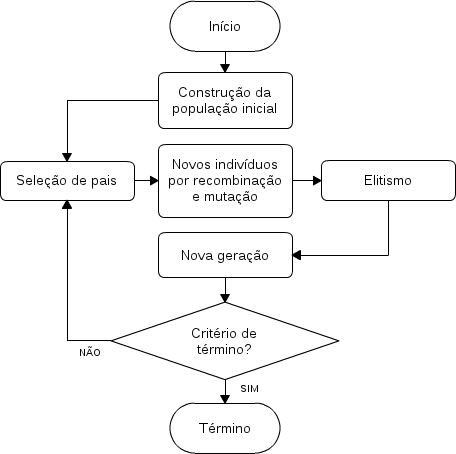
\includegraphics[width=0.51\textwidth]{../imgs/ga-ev.png}
\end{center} 
\end{frame}
\begin{frame}{Algoritmo evolucionário híbrido baseado na fertilização in vitro (IVF/EV-JB)}
\begin{center} 
  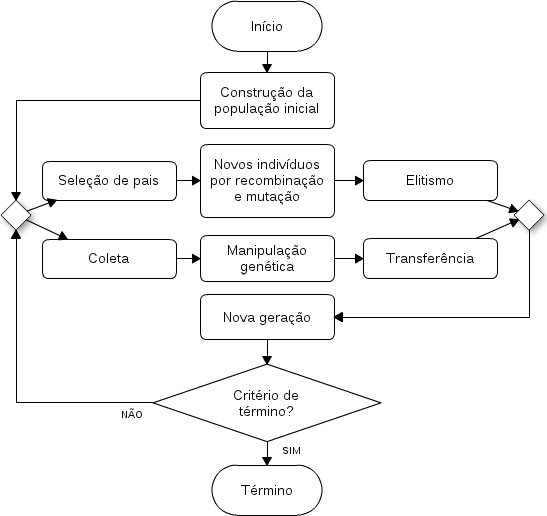
\includegraphics[width=0.52\textwidth]{../imgs/ivf-ev.png}
\end{center} 
\end{frame}

\subsection{Representação dos indivíduos}
\begin{frame}{Representação dos indivíduos}
Representação por chaves aleatórias (\textit{random-keys}):
\begin{center}
\paragraph{Seja $n = 2$ e $m = 4$, $S = \langle0.2, 0.5, 1.8, 6.7, 3.3, 2.4, 3.5, 2.4\rangle$}
\end{center}
\begin{enumerate}
\item<2-> $\langle0.2, 0.5, 1.8, 6.7, 3.3, 2.4, 3.5, 2.4\rangle \rightarrow \langle1, 2, 3, 8, 6, 4, 7, 5\rangle$;
\item<3-> $\langle1, 2, 3, 8, 6, 4, 7, 5\rangle \rightarrow \langle2, 1, 2, 1, 1, 1, 2, 2\rangle$,\\ com $S'_{i} = (S_{i}$ \textit{mod} $n) + 1$;
\item<4-> $S_{f} = \langle o_{2,1}, o_{1,1}, o_{2,2}, o_{1,2}, o_{1,3}, o_{1,4}, o_{2,3}, o_{2,4}\rangle$;\\
$o_{i,k}$: opera\c{c}\~{a}o da tarefa $i$ na $k$-\'{e}sima m\'{a}quina de sua configura\c{c}\~{a}o tecnol\'{o}gica.
\end{enumerate}
\end{frame}

\subsubsection{População inicial}
\begin{frame}{População inicial}
\begin{itemize}
\item<1-> Os indiv\'{i}duos--solu\c{c}\~{o}es da popula\c{c}\~{a}o inicial s\~{a}o criados a partir de distribui\c{c}\~{o}es normais
\item<2-> Cada dimens\~{a}o do vetor--indiv\'{i}duo \'{e} iniciada com o valor da distribui\c{c}\~{a}o $N(0, n \times m)$;
$n$ o n\'{u}mero de tarefas e $m$ o n\'{u}mero de m\'{a}quinas da oficina
\item<3-> Tamanho da população ($\mu$): $\mu = 2 \times n \times m$.
\end{itemize}
\end{frame}

\subsection{Mecanismos de seleção}
\begin{frame}{Mecanismos de seleção}
Mecanismos de seleção utilizados:
\begin{itemize}
\item<1-> Seleção por ranqueamento linear;
\item<2-> Seleção proporcional à aptidão; e
\item<3-> Seleção por torneio.
\end{itemize}
\end{frame}

\subsection{Mecanismos de recombinação}
\begin{frame}{Mecanismos de recombinação}
Mecanismos de recombinação utilizados:
\begin{itemize}
\item<1-> Recombinação de $1$--ponto;
\item<2-> Recombinaçaõ de $n$--pontos; e
\item<3-> Recombinação uniforme.
\end{itemize}
\end{frame}

\subsection{Mecanismos de mutação}
\begin{frame}{Mecanismos de seleção}
Dois mecanismos de mutação foram utilizados:
\begin{itemize}
\item<1-> Mutação por permutação; e
\item<2-> Geração aleatória de indivíduos
\begin{itemize}
\item<3-> Os 20\% piores indivíduos da população são substituídos por novos indivíduos construídos aleatoriamente
\end{itemize}
\end{itemize}
\end{frame}

\section{Análise dos resultados obtidos}
\begin{frame}{Análise dos resultados obtidos}
\begin{itemize}
\item<1-> Foram construídos 27 casos de experimentos a partir dos operadores de seleção e de variabilidade selecionados
\item<2-> As soluções algorítmicas têm como critério de parada a criação de 500 gerações populacionais, com exceção da população inicial
\end{itemize}
\end{frame}

\subsection{Efetividade da solução}
\begin{frame}{Efetividade da solução}
\begin{itemize}
\item<1-> Ambas as solu\c{c}\~{o}es desenvolvidas s\~{a}o solu\c{c}\~{o}es de qualidade por apresentarem respostas
pr\'{o}ximas ou semelhantes \`{a}quelas encontradas pela literatura
\item<2-> A m\'{e}dia populacional e os valores de pior indiv\'{i}duo do IVF/EV-JB corroboram com a motiva\c{c}\~{a}o
do algoritmo auxiliar paralelo (AAP) em manter qualidades genot\'{i}picas na popula\c{c}\~{a}o e prover resultados de
qualidade
\end{itemize}
\end{frame}

\subsection{Influência dos mecanismos de seleção e de variabilidade}
\begin{frame}{Influência dos mecanismos de seleção e de variabilidade}
\begin{itemize}
\item<1-> N\~{a}o foi poss\'{i}vel identificar quais s\~{a}o as reais influ\^{e}ncias dos operadores de variabilidade e de
sele\c{c}\~{a}o sobre a efetividade da solu\c{c}\~{a}o
\item<2-> Os resultados obtidos corroboram com o que é defendido na literatura: não existem operadores de seleção e variabilidade
ótimos \textit{per se}
\item<3-> As melhores configurações para a solução algorítmica construída são aquelas apresentadas nos experimentos
1, 2, 3, 25, 26, e 27
\end{itemize}
\end{frame}

\section{Conclusão}
\begin{frame}{Conclusão}
\begin{itemize}
\item Design de uma solução evolucionária
\item Importância da hibridização em contextos específicos
\item Importância da representação da solução
\item O algoritmo auxiliar paralelo baseado na fertilização in vitro e suas características identificadas
\end{itemize}
\end{frame}

\section{Referências Bibliográficas}
\begin{frame}[allowframebreaks]{Referências Bibliográficas}
\arial
\bibliographystyle{inf-ufg}
\bibliography{../bibliograph}
\end{frame}

\end{document}

